\documentclass[12pt]{article}
\usepackage{amsmath}
\usepackage{hyperref}
\usepackage[latin1]{inputenc}
\usepackage{graphicx}


\title{Zadanie 9}
\author{Wojciech Ganobis}
\date{21/24/20}

\begin{document}
Gestosc na naszym trojkacie wyraza sie wzorem:
$$f(x,y) = \frac{15}2 x^{2}y$$

\begin{figure}[h]
	\centering
   
		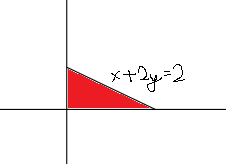
\includegraphics[width=8cm]{r1}
		\caption{XY}
\end{figure}
Prosta ograniczajaca to $x + 2y = 2$, mozemy ja sprawdzic obliczajac podwojna calke:
$$\int^{1}_{0}\int^{2-2y}_{0}\frac{15}2 x^{2}y dxdy = 1$$
Wiec jest ona poprawna.\\\\
Teraz wyznaczmy $T$ i dodajmy $Z$, gdzie $T = \frac{X}Y$ i $Z = Y$\\
Po przeksztalceniu otrzymujemy $X = TZ$ i $Y = Z$\\
Obliczmy:
$$\frac{\partial (X,Y)}{\partial (T,Z)} = \left|\begin{array}{cc}
\frac{\partial X}{\partial T} & \frac{\partial X}{\partial Z} \\
\frac{\partial Y}{\partial T} & \frac{\partial Y}{\partial Z}
\end{array}\right| = \left|\begin{array}{cc}
Z &T \\
0 & 1
\end{array}\right| = Z$$\\
Funkjca gestosci g:
$$g(z,t) = f(x(z,t), y(z,t)) * \|J\| = \frac{15}2 t^{2}z^{2} * z * z = t^{2}z^{4}$$\\
Teraz kilka prostych przeksztalcen:\\
$$0 \leq Y \leq 1,    0 \leq X \leq 2-2Y$$
$$0 \leq Z \leq 1,    0 \leq TZ \leq 2-2Y$$
$$0 \leq Z \leq 1,    0 \leq Z \leq \frac{Z}{T+2}$$
Bierzemy pod uwage tylko 2 rownanie poniewaz jest "bardziej ograniczajace", wiec obliczamy calke:
$$\int^{\frac{2}{t+2}}_{0}\frac{15}2 t^{2}z^{z}dz = \frac{48t^{2}}{(t+2)^5}$$\\
Nasza funkcja gestosci to $\frac{48t^{2}}{(t+2)^5}$\\
Mozemy jeszcza ja sprawdzic obliczajac calke:
$$\int^{\inf}_{0}\frac{48t^{2}}{(t+2)^5}dt = 1$$
 
\end{document}
